\setcounter{chapter}{0}
\setcounter{section}{0}
\begin{center}
\chapter{\tenchuongi}
\end{center}

%===================================================================
\section{Khái quát về CNN}
\subsection{Giới thiệu}
Tương tự như việc trẻ em học cách nhận diện đối tượng, chúng ta cần cho thuật toán học rất nhiều hình ảnh trước khi nó có thể đưa ra phân loại cho hình ảnh đầu vào mà nó chưa từng thấy \cite{ntt8b3}.

\begin{figure}[H]
	\centering
	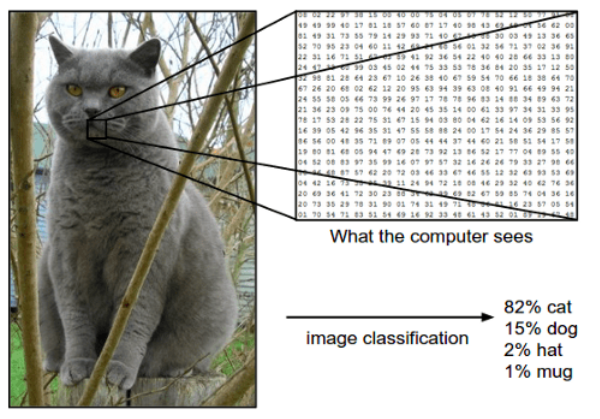
\includegraphics[width=0.7\linewidth]{images/how_computer_see_image}
	\caption[Cách máy tính "nhìn" một hình.]{Cách máy tính "nhìn" một hình.}
	%\label{fig:howcomputerseeimage}
\end{figure}

Máy tính “nhìn” theo cách khác con người. Trong thế giới máy tính chỉ có những con số. Mỗi hình ảnh có thể được biểu diễn dưới dạng mảng 2 chiều những con số được gọi là các pixel.

Mặc dù máy tính nhìn nhận theo cách khác con người, chúng ta vẫn có thể dạy máy tính nhận diện các mẫu như con người. Điều quan trọng là chúng ta cần nghĩ về hình ảnh theo một cách khác đi.

Để dạy thuật toán nhận diện đối tượng trong hình ảnh, ta sử dụng một loại mạng ANN, đó là CNN. Tên của nó được dựa trên phép tính quan trọng được sử dụng trong mạng- tích chập.

Mạng CNN lấy cảm hứng từ não người. Nghiên cứu trong những thập niên 1950 và 1960 của D.H Hubel và T.N Wiesel trên não của động vật đã đề xuất một mô hình mới cho việc cách mà động vật nhìn nhận thế giới. Trong báo cáo, hai ông đã diễn tả 2 loại tế bào nơ-ron trong não và cách hoạt động khác nhau: tế bào đơn giản (simple cell – S cell) và tế bào phức tạp (complex cell – C cell). 

Các tế bào đơn giản được kích hoạt khi nhận diện các hình dáng đơn dản như đường nằm trong một khu vực cố định và một góc cạnh của nó. Các tế bào phức tạp có vùng tiếp nhận lơn hơn và đầu ra của nó không nhạy cảm với những vị trí cố định trong vùng. 

Trong thị giác, vùng tiếp nhận của một nơ-ron tương ứng với một vùng trên võng mạc nơi mà sẽ kích hoạt nơ-ron tương ứng. 

Năm 1980, Fukushima đề xuất mô hình mạng nơ-ron có cấp bậc gọi là neocognitron. Mô hình này dựa trên khái niệm về S cell và C cell. Mạn neocognitron có thể nhận diện mẫu dựa trên việc học hình dáng của đối tượng. 

Sau đó vào năm 1998, mạng CNN được giới thiệu bởi Bengio, Le Cun, Bottou và Haffner. Mô hình đầu tiên của họ được gọi tên là LeNet-5. Mô hình này có thể nhận diện chữ số viết tay.

\subsection{Kiến trúc mạng CNN}
Mạng CNN có kiến trúc khác với Mạng Nơ-ron thông thường. Mạng ANN bình thường chuyển đổi đầu vào thông qua hàng loạt các tầng ẩn. Mỗi tầng là một tập các nơ-ron và các tầng được liên kết đầy đủ với các nơ-ron ở tầng trước đó. Và ở tầng cuối cùng sẽ là tầng kết quả đại diện cho dự đoán của mạng.

Đầu tiên, mạng CNN được chia thành 3 chiều: rộng, cao, và sâu. Kế đên, các nơ ron trong mạng không liên kết hoàn toàn với toàn bộ nơ-ron kế đến nhưng chỉ liên kết tới một vùng nhỏ. Cuối cùng, một tầng đầu ra được tối giản thành véc-tơ của giá trị xác suất (hình \ref{fig:neuronnetwork}).

\begin{figure}[H]
	\centering
	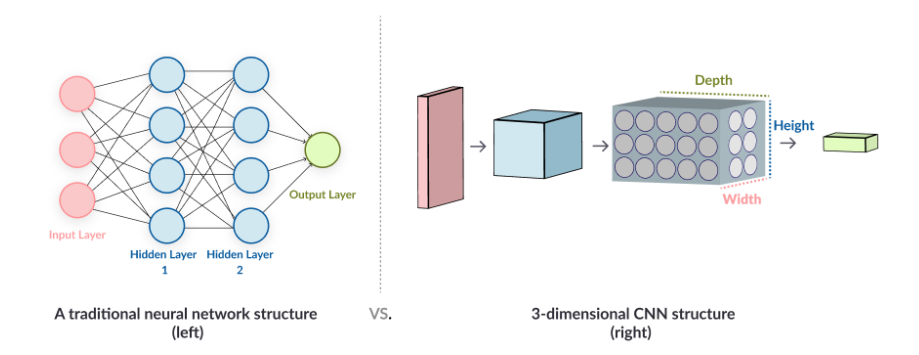
\includegraphics[width=1\linewidth]{images/neuronnetwork}
	\caption{Mạng Neuron thông thường (trái) và CNN (phải).}
	\label{fig:neuronnetwork}
\end{figure}

Mạng CNN gồm hai thành phần:

\indent\indent \textbf{Phần tầng ẩn hay phần rút trích đặc trưng:} trong phần này, mạng sẽ tiến hành tính toán hàng loạt phép tích chập và phép hợp nhất (pooling) để phát hiện các đặc trưng. Ví dụ: nếu ta có hình ảnh con ngựa vằn, thì trong phần này mạng sẽ nhận diện các sọc vằn, hai tai, và bốn chân của nó.

\indent\indent  \textbf{Phần phân lớp:} tại phần này, một lớp với các liên kết đầy đủ sẽ đóng vai trò như một bộ phân lớp các đặc trưng đã rút trích được trước đó. Tầng này sẽ đưa ra xác suất của một đối tượng trong hình \ref{fig:kientruccnn}.
\begin{figure}[H]
	\centering
	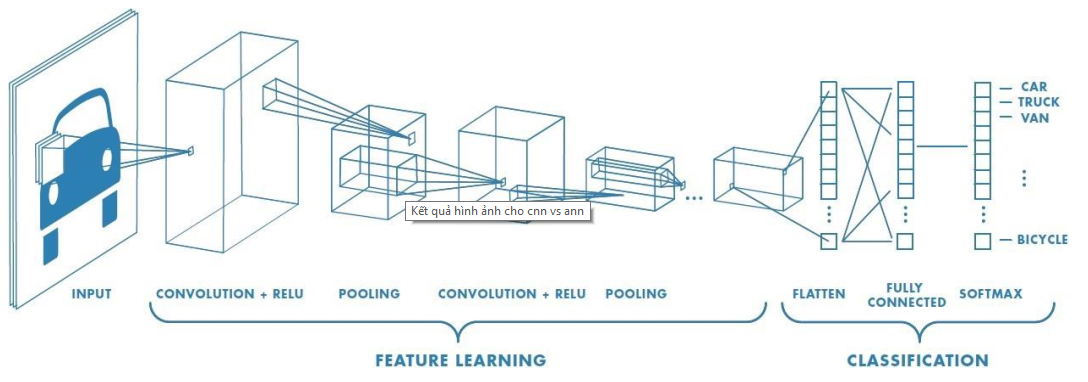
\includegraphics[width=1\linewidth]{images/kientruccnn}
	\caption{Kiến trúc mạng CNN.}
	\label{fig:kientruccnn}
\end{figure}

\subsubsection{Trích rút đặc trưng}
\paragraph{Lớp tích chập}
Tích chập là một khối quan trọng trong CNN. Thuật ngữ tích chập được dựa trên một phép hợp nhất toán học của hai hàm tạo thành hàm thứ ba. Phép toán này kết hợp hai tập thông tin khác nhau.

Trong trường hợp CNN, tích chập được thực hiện trên giá trị đầu vào của dữ liệu và kernel/filter (thuật ngữ này được sử dụng khác nhau tùy tình huống) để tạo ra một bản đồ đặc trưng (feature map). 

Ta thực hiện phép tích chập bằng cách trượt kernel/filter theo dữ liệu đầu vào. Tại mỗi vị trí, ta tiến hành phép nhân ma trận và tính tổng các giá trị để đưa vào bản đồ đặc trưng. Thao tác này đã được minh họa cụ thể trong hình \ref{fig:padding18}

\begin{figure}[H]
	\centering
	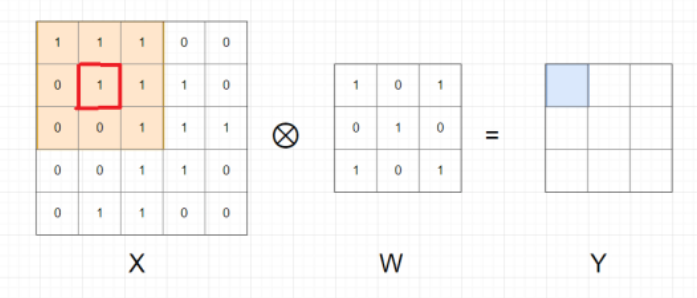
\includegraphics[width=1\linewidth]{images/padding18.png}
	\caption{Minh họa phép tích chập.}
	\label{fig:padding18}
\end{figure}

Trong thực tế, tích chập được thực hiện hiện trên không gian 3 chiều. Vì mỗi hình ảnh được biểu diễn dưới dạng 3 chiều: rộng, cao, và sâu. Chiều sâu ở đây chính là giá trị màu sắc của hình (RGB).

Ta thực hiện phép tích chập trên đầu vào nhiều lần khác nhau. Mỗi lần sử dụng một kernel/filter khác nhau. Kết quả ta sẽ thu được những bản đồ đặc trưng khác nhau. Cuối cùng, ta kết hợp toàn bộ bản đồ đặc trưng này thành kết quả cuối cùng của tầng tích chập.

\paragraph{Lớp ReLU}

Tương tự như mạng nơ-ron thông thường, ta sử dụng một hàm kích hoạt (activate function) để có đầu ra dưới dạng phi tuyến. Trong trường hợp CNN, đầu ra của phép tích chập sẽ đi qua hàm kích hoạt nào đó ví dụ như hàm tinh chỉnh các đơn vị tuyến tính (Rectified linear units - ReLU). 

Trong quá trình trượt kernel/filter trên dữ liệu đầu vào, ta sẽ quy định một bước nhảy (stride) với mỗi lần di chuyển. Thông thường ta lựa chọn thường chọn bước nhảy là 1. Nếu kích thước bước nhảy tăng, kernel/filter sẽ có ít ô trùng lắp.

Bởi vì kích thước đầu ra luôn nhỏ hơn đầu vào nên ta cần một phép xử lí đầu vào để đầu ra không bị co giãn. Đơn giản ta chỉ cần thêm một lề nhỏ vào đầu vào. Một lề (padding) với giá trị 0 sẽ được thêm vào xung quanh đầu vào trước khi thực hiện phép tích chập. 

\paragraph{Lớp pooling}

Thông thường, sau mỗi tầng tích chập, ta sẽ cho kết quả đi qua một tầng hợp nhất (pooling layer). Mục đích của tầng này là để nhanh chóng giảm số chiều. Việc này giúp giảm thời gian học và hạn chế việc overfitting. 

Một phép hợp nhất đơn giản thường được dùng đó là max pooling, phép này lấy giá trị lớn nhất của một vùng để đại diện cho vùng đó. Kích thước của vùng sẽ được xác định trước để giảm kích thước của bản đồ đặc trưng nhanh chóng nhưng vẫn giữ được thông tin cần thiết (hình \ref{fig:maxpooling22}).

\begin{figure}[H]
	\centering
	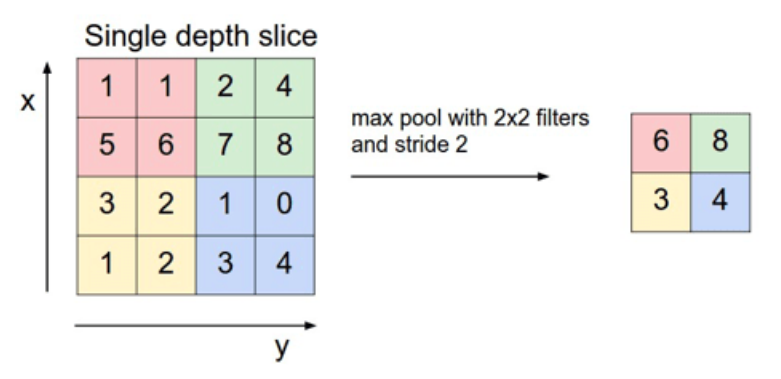
\includegraphics[width=0.8\linewidth]{images/maxpooling22.png}
	\caption{Max pooling kích thước 2×2}
	\label{fig:maxpooling22}
\end{figure}

Như vậy, khi thiết kế phần rút trích đặc trưng của mạng CNN, ta cần chú ý đến 4 siêu tham số quan trọng là: Kích thước kernel/filter, Số lượng kernel/filter, Kích thước bước nhảy (stride), Kích thước lề (padding).

\subsubsection{Phân lớp}
Trong phần phân lớp, ta sử dụng một vài tầng với kết nối đầy đủ để xử lí kết quả của phần tích chập. Vì đầu vào của mạng liên kết đầy đủ là 1 chiều, ta cần làm phẳng đầu vào trước khi phân lớp. Tầng cuối cùng trong mạng CNN là một tầng liên kết đầy đủ, phần này hoạt động tương tự như mạng nơ-ron thông thường.

Kết quả thu được cuối cùng cũng sẽ là một véc-tơ với các giá trị xác suất cho việc dự đoán như mạng nơ-ron thông thường.

\begin{figure}[H]
	\centering
	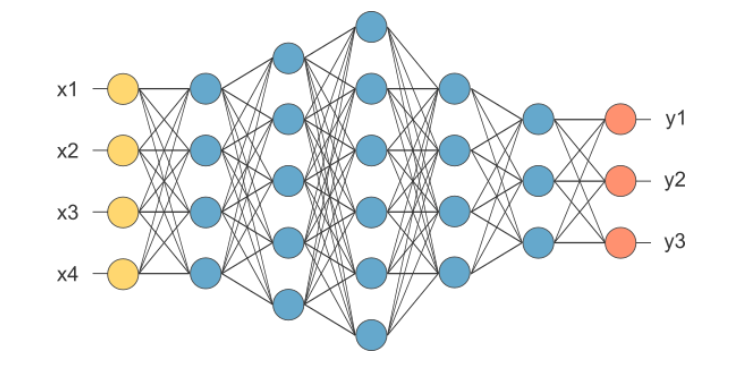
\includegraphics[width=0.8\linewidth]{images/fullyconnected.png}
	\caption{Lớp kết nối đầy đủ}
\end{figure}

\subsection{Ứng dụng CNN trong phân loại ảnh}

